\documentclass[10pt]{beamer}
\beamertemplatenavigationsymbolsempty
\usecolortheme{beaver}
\setbeamertemplate{blocks}[rounded=true, shadow=true]
%\setbeamertemplate{footline}[page number]

\usepackage[utf8]{inputenc}
\usepackage[english,russian]{babel}
\usepackage{amssymb,amsfonts,amsmath,mathtext}
\usepackage{subfig}
\usepackage[all]{xy}
\usepackage{array}
\usepackage{multicol}
\usepackage{hyperref}
\usepackage{hhline}
\usepackage{caption}
\usepackage{subfig}

\DeclareMathOperator*{\argmax}{arg\,max}
\DeclareMathOperator*{\argmin}{arg\,min}

\graphicspath{ {../figures/} }

%----------------------------------------------------------------------------------------------------------
\title[\hbox to 56mm{Восстановление снимков фМРТ}]{Восстановление снимков фМРТ \\ по просматриваемому видеоряду}
\author[Н.\,С.~Киселев]{Никита Сергеевич Киселев}
\institute{Московский физико-технический институт}
\date{\footnotesize
\par\smallskip\emph{Курс:} Автоматизация научных исследований\par/Группа 003
\par\smallskip\emph{Эксперт:} А.\,В.~Грабовой
\par\bigskip\small 2023}
%----------------------------------------------------------------------------------------------------------
\begin{document}
%----------------------------------------------------------------------------------------------------------
\begin{frame}{Neural Networks Loss Landscape Convergence in Different Low-Dimensional Spaces}

\textbf{Goal:} Measure how the loss function changes as the training set size grows:
\[
\Delta_k = \mathbb{E}_{p(\mathbf{w})}\Bigl(\mathcal{L}_{k}(\mathbf{w}) - \mathcal{L}_{k-1}(\mathbf{w})\Bigr)^2.
\]

\textbf{Method:}
\begin{itemize}
    \item \textbf{Monte Carlo:} Generate points near the minimum according to $p(\mathbf{w})$ and average the differences.
    \item \textbf{Hessian Eigenvectors:} Use directions with the largest eigenvalues to focus on key curvature components.
\end{itemize}

\begin{columns}[t]
    \column{0.35\textwidth}
    \centering
    \hspace*{-2cm}
    \includegraphics[width=0.95\textwidth]{img/LS_16.jpg}\\
    \hspace*{-2cm}
    \scriptsize \textit{Loss function}

    \column{0.47\textwidth}
    \centering
    \vspace*{-3.3cm}
    \hspace*{-2.2cm}
    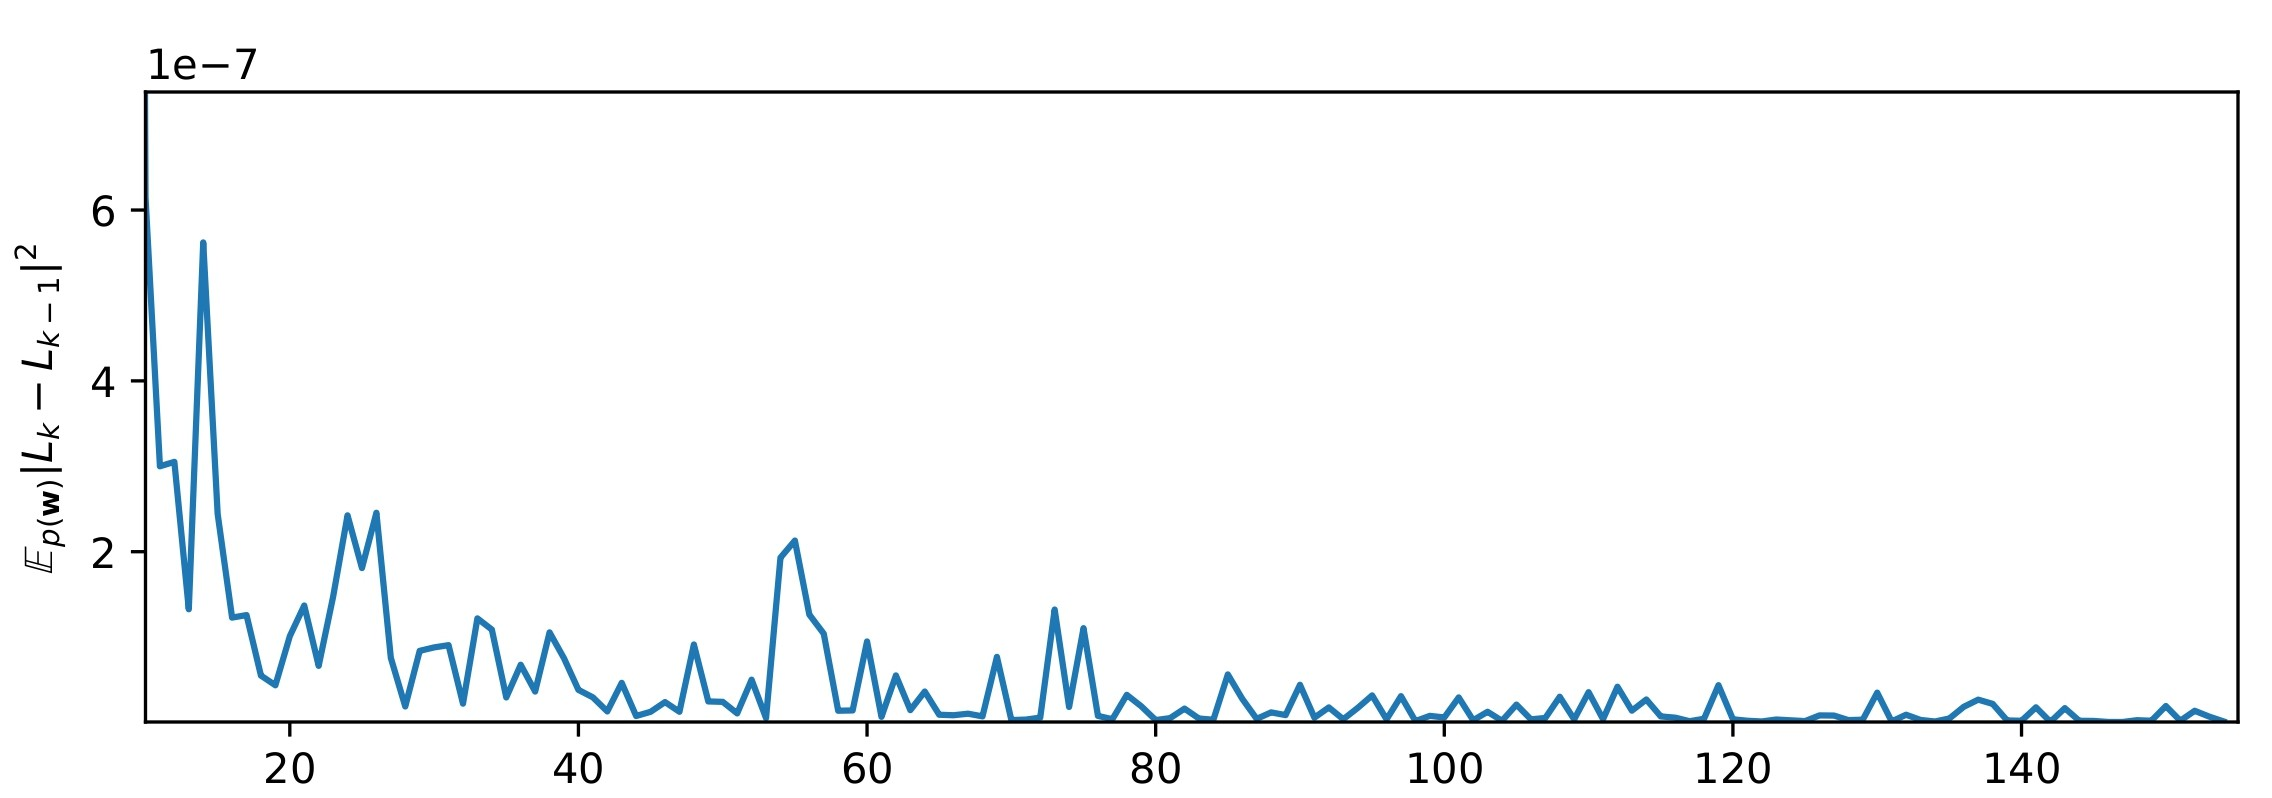
\includegraphics[width=1.6\textwidth]{img/D_32.jpg}\\
    \hspace*{-1.2cm}
    \scriptsize \textit{$\Delta_k$ function}
\end{columns}

\end{frame}
%----------------------------------------------------------------------------------------------------------
\end{document}
